\chapter{给圆盘找一条路：配置空间与 A*}
\begin{notebox}
\textbf{目标}\quad 将圆盘规划化成中心点搜索，理解栅格、未知区域、路径与轨迹的区别。\\
\textbf{先修}\quad 第 03、07 章。先在给定栅格上检查算法，再接观测地图。
\end{notebox}

\section{先运行一张带窄门的地图}
\begin{lstlisting}[language=bash]
ros2 run motion2d astar_demo tmp/ch11_astar
/usr/bin/python3 scripts/plot_ch11_astar.py
\end{lstlisting}
这次输入是手工给定的 $41\times31$ 栅格，分辨率 0.1 m。
中间隔墙有宽 0.7 m 的门；起点 $(.75,.75)$ m，终点 $(3.25,2.25)$ m。
改变半径，观察门从可通行变成不可达。该小实验隔离规划算法，不冒充未知环境建图。

\section{圆盘变成一个中心点}
设原始阻塞区域为 $\mathcal O$，圆盘物理半径为 $r$，额外安全裕量为 $m$。
中心点必须避开膨胀集合
\begin{equation}
\mathcal O_{\rm conf}=\mathcal O\oplus B(0,r+m).
\end{equation}
这里 $\oplus$ 表示将集合中的每个点向外扩张一个半径 $r+m$ 的圆。
半径与裕量只加一次；后面使用已经膨胀的地图时不能再重复扣除机器人半径。

原始占据栅格表示方格的\textbf{面积}，不是只有格子中心的一个点。
本章还要求输出自由格的整个闭区域都安全，方便后续构造走廊。
两个边长 $\rho$ 的格子，相对索引差为 $(\Delta i,\Delta j)$，其最小距离为
\begin{equation}
d_x=\rho\max(0,|\Delta i|-1),\qquad
 d_y=\rho\max(0,|\Delta j|-1),\qquad d=\sqrt{d_x^2+d_y^2}.
\end{equation}
若 $d\leq r+m$，候选格子被阻塞。相邻方格共享边或角时距离为零；接触也视为碰撞。
\lstinputlisting[language=C++,linerange={inflation_stencil_begin-inflation_stencil_end},
  includerangemarker=false]{../ros2_ws/src/motion2d/src/planning/inflation.cpp}

这种整格安全证书比只检查中心更保守。即使 $r=0$，与障碍接触的相邻格仍会被排除。
连续几何可以通过的窄门，粗网格可能判不可达；缩小 $\rho$ 能减少这类保守损失。
地图外部也视为阻塞，边界附近格子同样要满足距离要求。

\section{A* 的三个数与两种邻接}
$g(n)$ 是从起点到节点 $n$ 已知的最小代价，$h(n)$ 是到目标的下界，优先展开
\begin{equation} f(n)=g(n)+h(n). \end{equation}
四邻接每步长 $\rho$，使用 Manhattan 距离；八邻接另有长 $\sqrt2\rho$ 的对角步，使用 octile 距离。
设到目标的索引差绝对值为 $d_x,d_y$，则
\begin{align}
h_4 &= \rho(d_x+d_y),\\
h_8 &= \rho\bigl[\max(d_x,d_y)+(\sqrt2-1)\min(d_x,d_y)\bigr].
\end{align}
无障碍时这就是最短距离；障碍只会让路更长，因此不会高估。
它们还满足一致性，节点确定后不必反复重新打开。

\lstinputlisting[language=C++,linerange={astar_neighbors_begin-astar_neighbors_end},
  includerangemarker=false]{../ros2_ws/src/motion2d/src/planning/astar.cpp}

关键是中间的对角检查：终点自由不代表连线安全。
例如右邻格被堵、上邻格自由，即使右上格自由，也不能沿对角线擦过右邻障碍的角。
\textbf{练习 ch11-1} 补完 diagonal\_step.hpp，分别检查两侧被挡的情况。

程序保留每个节点的父节点，从目标反向回溯，再反转得到格子序列。
输出折线包含精确请求的起终点；它们可以不在格子中心。
因为起终格的整个面积已保证安全，格内接到中心的短线仍然安全。
两个点在同一格时直接相连，不必绕到格子中心。

\clearpage
\section{未知不是免费的捷径}
只有已观测且概率编码不大于 35 的格子作为原始自由格；未知 $-1$、不确定与占据均默认阻塞。
这是本课程的规划策略，不是 ROS 强制规定。显式设置 unknown\_blocked=false 可以做乐观探索实验，
但不能把未观测空间称为已验证安全。

搜索结果必须区分：
\begin{center}\small
\begin{tabular}{ll}\toprule
状态 & 含义 \\\midrule
found & 在当前栅格和规则下找到路径 \\
invalid\_start / invalid\_goal & 起点或终点越界、被堵或接触阻塞边界 \\
unreachable & 两点有效，但自由格图不连通 \\\bottomrule
\end{tabular}
\end{center}
失败时返回空路径和无穷大代价。成功的 grid\_cost 是\textbf{中心节点图}上的最短距离，
不是含精确端点及后续简化的折线总长。两者的定义不能混用。

\section{删掉折点之前，检查整条线段}
贪心简化从当前点开始，寻找能直视的最远后续点，再继续。
这是减少折点的实用方法，不保证连续空间的全局最短路线。
检查线段 $p(t)=a+t(b-a)$，$t\in[0,1]$ 与每个候选阻塞方格的闭区间是否相交。
对每个轴施加 $l\leq p(t)\leq u$，把允许的 $t$ 区间相交；非空就是接触或穿过障碍。

本实现遍历线段包围框中的格子，采用解析区间裁剪。它检查细障碍、擦角和沿边接触，
不用固定间距采样“猜测安全”。代价是长斜线可能检查较多格子；之后可优化为 supercover DDA，
但应保留当前实现作为容易审查的对照。

\begin{notebox}
\textbf{建图射线遍历不能直接当作碰撞检查}\quad 第七章 DDA 在恰好经过角点时同时跨两个轴，
跳过只被角点触到的旁边格子。这适合那里的观测更新约定，但会漏掉规划中的角点接触。
相同的网格不表示相同的遍历语义。
\end{notebox}

\textbf{常见错误：}只看对角终点；把未知默认当作自由；只查简化线段上的少量采样点；
扩大半径后仍使用旧的膨胀图；将找到的一串点当成满足速度、加速度和控制约束的轨迹。
本章输出只有几何折线，时间分配和连续曲线将在第十四章开始。

\clearpage
\section{半径、邻接与窄门实验}
\begin{figure}[h]
\centering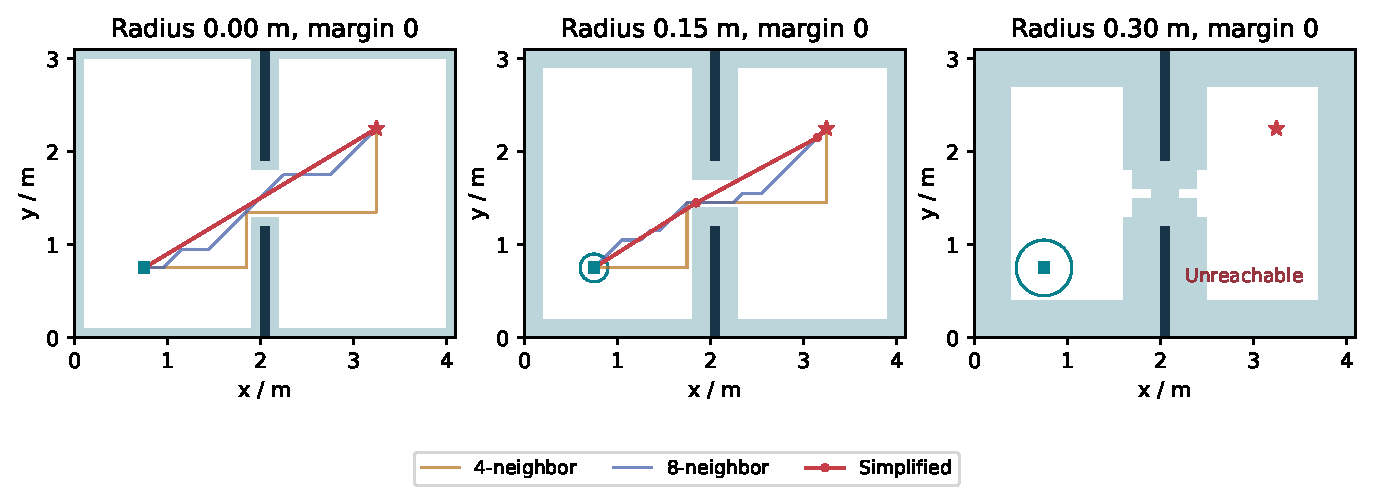
\includegraphics[width=\linewidth]{figures/ch11_astar.pdf}
\caption{深色是给定隔墙，浅蓝是额外阻塞的配置空间格子，白色可规划。
绿方块为起点，红星为目标；绿圆保持真实半径与坐标等比例。红线为八邻接结果的简化。}
\end{figure}
\begin{center}\small
\pgfplotstabletypeset[col sep=comma,
columns={radius,neighbors,status,grid_cost,expanded,simplified_points},
columns/radius/.style={column name=半径/m},columns/neighbors/.style={column name=邻接},
columns/status/.style={column name=状态,string type,string replace*={found}{找到},string replace*={unreachable}{不可达}},
columns/grid_cost/.style={column name=图代价/m,string type,string replace*={inf}{---}},
columns/expanded/.style={column name=扩展节点},columns/simplified_points/.style={column name=简化点数},
every head row/.style={before row=\toprule,after row=\midrule},
every last row/.style={after row=\bottomrule}]{data/ch11_astar.csv}
\end{center}
本实验裕量为零，半径分别为 0、0.15、0.30 m。四邻接成功时图代价为 4 m，
八邻接约为 3.12132 m。两种半径的成功代价相同不表示路径完全相同：栅格中可以存在多个等长路线。
扩展节点数同时受启发式、可用区域和并列排序影响，不能当作一般性能承诺。

0.7 m 门能在连续几何中容纳直径 0.6 m 的圆盘，但本例找不到整格都安全的贯通路径。
这是明确的离散保守性，不是把真实机器人偷偷变大；分辨率、半径与整格安全要求共同决定结果。
下一步接入观测地图后，还要区分几何变窄与尚未看见造成的封闭。

\begin{enumerate}
\item \textbf{理解：}在小网格上手算 $g,h,f$，解释四邻接与八邻接启发式的不同。
\item \textbf{代码：}完成邻居检查，覆盖外边界、两侧被挡和合法对角。
\item \textbf{实验：}改变半径、分辨率或未知策略，记录可达性、代价与简化点数。
\end{enumerate}
\textbf{验收：}30 组 seed=1111 随机栅格与独立 Dijkstra 的最短代价一致；
另检查已知四/八邻接距离、精确端点、同格路径、窄门、未知、外界、穿角、线段擦边/擦角与简化后安全。
ROS 观测地图和点击目标在下一功能接入。
